    导航就字面上说,就是引导航行的意思,而其确切的定义可表述为:导航是有目的地、
    安全有效地引导运动体(船只、潜艇、地面车辆以及飞机、宇宙飞船等). 也就是在当前位置已知的前提下,
    计算如何才能到达目的地,也即路径规划。本系统设计的导航子系统(navigator)执行流程如图\ref{fig:navigator}所示.
    \begin{figure}[htbp]
        \centering
        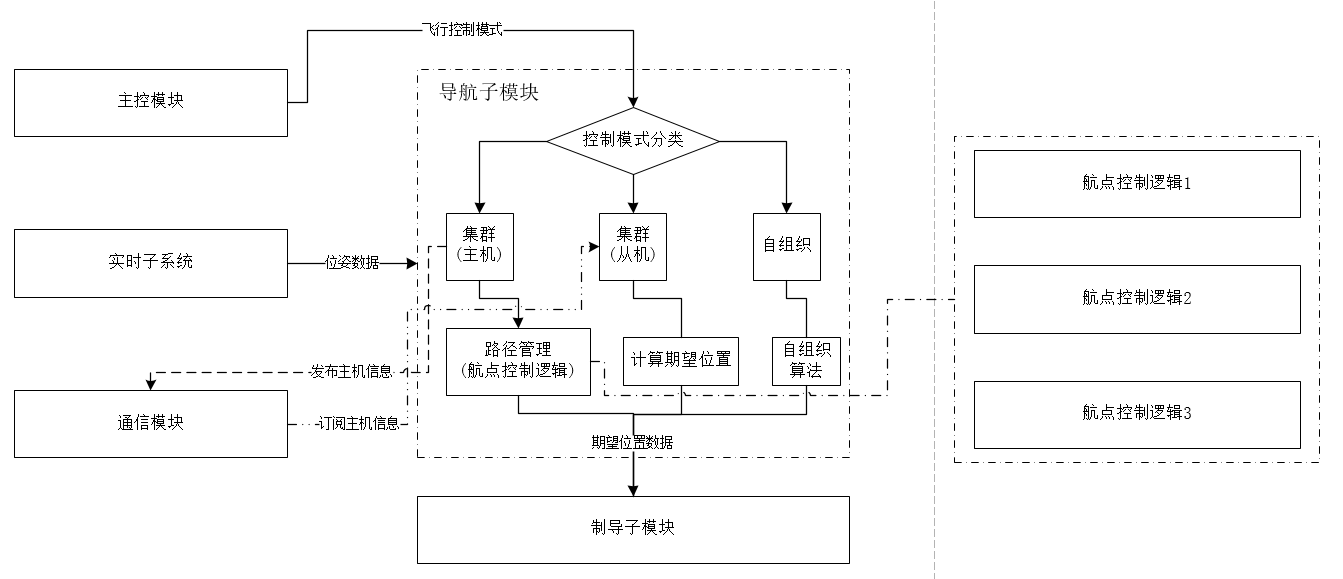
\includegraphics[width=\textwidth]{pictures/navigator.png}
        \caption{navigator}
        \label{fig:navigator}
    \end{figure}
    路径管理内部有三处控制逻辑, 分别对应着直线切换, 转弯圆角, 以及dubins曲线三种控制算法. 会在后面"算法"一节中进行介绍. 

